% ---------------------------------------------------------------
% PRESENTATION TEMPLATE FOR THE II CLIV
% Last update July 4, 2018 by Gabriel B. Martins
% ---------------------------------------------------------------

\documentclass[12pt,handout]{beamer}
\usepackage{graphicx,url}
\usepackage[brazil]{babel}
\usepackage[utf8]{inputenc}
\batchmode
\usepackage{helvet}
\usepackage{amsmath,amssymb,enumerate,epsfig,bbm,calc,color,ifthen,capt-of}


\usebackgroundtemplate{
	
\includegraphics[height=\paperheight]{./figures/bg.png}
}

% ---------------------------------------------------------------
% Predefined colors
% ---------------------------------------------------------------
\definecolor{BaseColor}{RGB}{102,45,145}
\usecolortheme[named=BaseColor]{structure}

% ---------------------------------------------------------------
% Beamer template
% ---------------------------------------------------------------
\defbeamertemplate*{footline}{infolines theme}
{
	\leavevmode
	\hbox{
	
	\begin{beamercolorbox}[wd=0.1\paperwidth,ht=3ex,dp=1ex,center]{author in head/foot}
	
	\end{beamercolorbox}

	\begin{beamercolorbox}[wd=0.81\paperwidth,ht=2.25ex,dp=2ex,center]{title in head/foot}
		\usebeamerfont{title in head/foot}\textcolor{BaseColor}{III Congresso Latino Americano de Engenharia do Vento}
	\end{beamercolorbox}


	\begin{beamercolorbox}[wd=.09\paperwidth,ht=2.25ex,dp=1ex,left]{date in head/foot}
		\usebeamerfont{page number in head/foot} 
		\insertframenumber{}  
	\end{beamercolorbox}}

	\vskip0pt

}

\makeatletter
\setbeamertemplate{frametitle}{
    \ifbeamercolorempty[bg]{frametitle}{}{\nointerlineskip}%
    \@tempdima=\textwidth%
    \advance\@tempdima by\beamer@leftmargin%
    \advance\@tempdima by\beamer@rightmargin%
    \hspace*{0.8cm} %%%%%%%%%%%%% For example insert shift to right
    \begin{beamercolorbox}[sep=0.3cm,left,wd=\the\@tempdima]{frametitle}
        \usebeamerfont{frametitle}%
        \vbox{}\vskip-1ex%
        \if@tempswa\else\csname beamer@ftecenter\endcsname\fi%
        \strut\insertframetitle\strut\par%
        {%
            \ifx\insertframesubtitle\@empty%
            \else%
            {\usebeamerfont{framesubtitle}\usebeamercolor[fg]{framesubtitle}\insertframesubtitle\strut\par}%
            \fi
        }%
        \vskip-1ex%
        \if@tempswa\else\vskip-.3cm\fi% set inside beamercolorbox... evil here...
    \end{beamercolorbox}%
}
\makeatother

\setbeamersize{text margin left=1.2cm}
\setlength{\parskip}{\baselineskip} 

% ---------------------------------------------------------------
% Title and author (must be edited)
% ---------------------------------------------------------------
\title[LOW COST ANEMOMETERS]{LOW COST ANEMOMETERS FOR WIND TUNNEL AND VENTILATION APPLICATIONS}

\author{Paulo Jabardo\inst{a}$^\dagger$ \and Leandro Alves\inst{a} \and Gabriel Borelli\inst{a} \and Gilder Nader} %The speaker must be pointed with a dagger or an asterisk

\institute{
	\inst{a}
	Institute for Technological Research, São Paulo, Brazil 
}

\date{\scriptsize{\textcolor{BaseColor}{III CONGRESSO LATINO AMERICANO DE ENGENHARIA DO VENTO \\ \vspace{0.3cm} SÃO PAULO, 2018}}}

\logo{
\includegraphics[height=1.5cm]{./figures/CLIV_logo.pdf}\vspace{-0.5cm}}


% ---------------------------------------------------------------
% Document starts here
% ---------------------------------------------------------------

\begin{document}

% ---------------------------------------------------------------
% Title page
% ---------------------------------------------------------------

\begin{frame}
	\titlepage
\end{frame}

% ---------------------------------------------------------------
% Presentation slides
% ---------------------------------------------------------------

\begin{frame}
	\frametitle{Motivação}
	\framesubtitle{Sensor de Irwin e tubos de Pitot não bastam???}
	
        Tubos de Pitot em diferentes tamanhos e formas têm sido utilizados faz séculos em tudo quanto é laboratório! 
	
	\begin{itemize}
		\item Como medir velocidades baixas ($< 4 m/s$)?
		\item Como medir várias velocidades simultaneamente?
		\item Como adquirir isso no computador? Ou celular?
                \item Como qualquer um pode fazer isso?
                \item Como fazer tudo acima a baixo custo?
	\end{itemize}
\end{frame}

\begin{frame}
  \frametitle{Termo-anemômetros}

  Princípio básico: transferência de calor por convecção varia com a velocidade

  Um corpo aquecido em equilíbrio:
  \[
  h(U)\cdot A \cdot(T_w - T_a) = R\cdot i^2
  \]
  Uma maneira efetiva:
  \[
  R = R(T_w)
  \]
  
\end{frame}

\begin{frame}
  \frametitle{Termistor}
  Dispositivo semi-condutor
  \[
  R = R_0\exp\left[ B \cdot \left(\frac{1}{T} - \frac{1}{T_0} \right) \right]
  \]
  \centering
  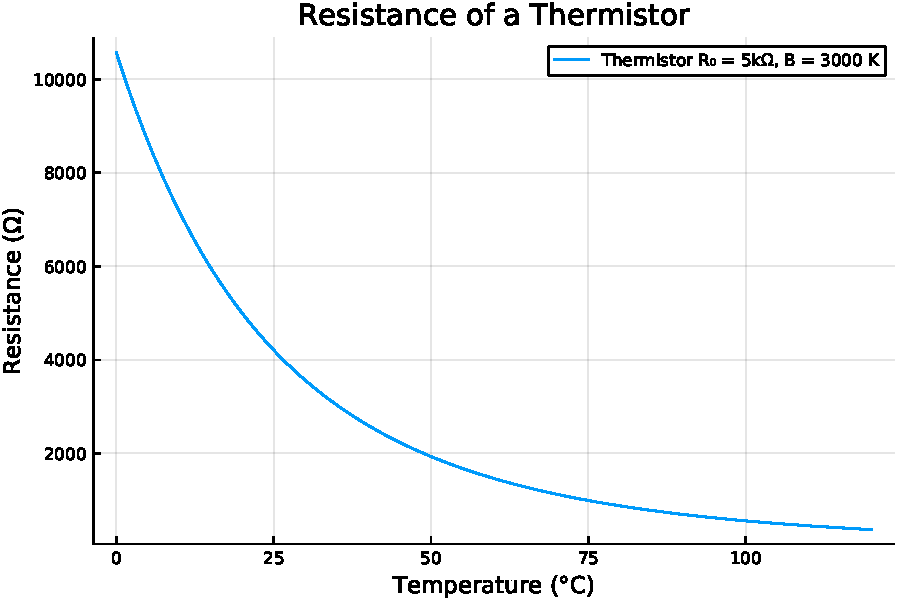
\includegraphics[height=0.7\textheight]{../../figures/thermistor.pdf}
  
\end{frame}


\begin{frame}
  \frametitle{Termistor}
  \framesubtitle{Exemplo de termistor facilmente encontrado  no mercado} 
  \centering
  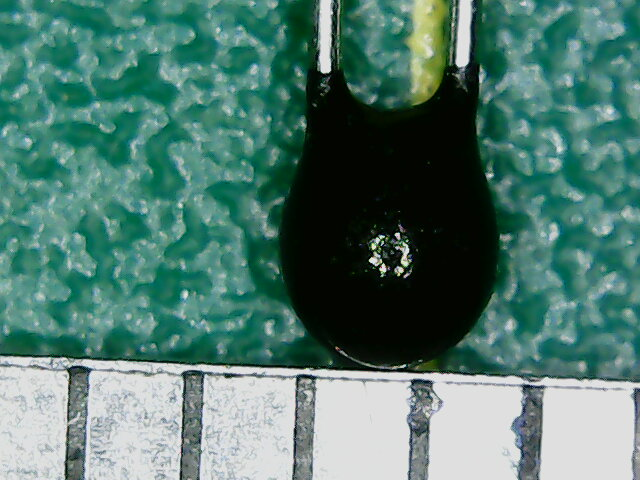
\includegraphics[height=0.7\textheight]{../../figures/termistor.jpg}
\end{frame}

\begin{frame}
  \frametitle{Termo-anemômetro a corrente constante}
  \framesubtitle{Mais simples impossível!}
  \centering
  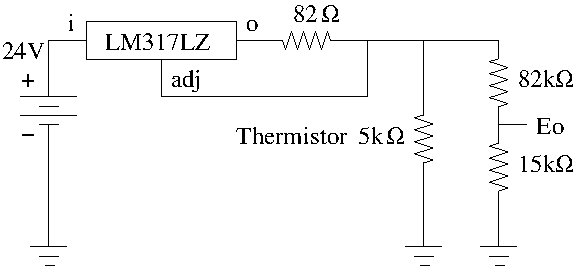
\includegraphics[width=0.66\textwidth]{../../figures/cca.pdf} 
  
\end{frame}

\begin{frame}
  \frametitle{Termo-anemômetro a corrente constante (CCA)}
  \framesubtitle{Simulação da operação}
 \centering
  \begin{tabular}{cc}
    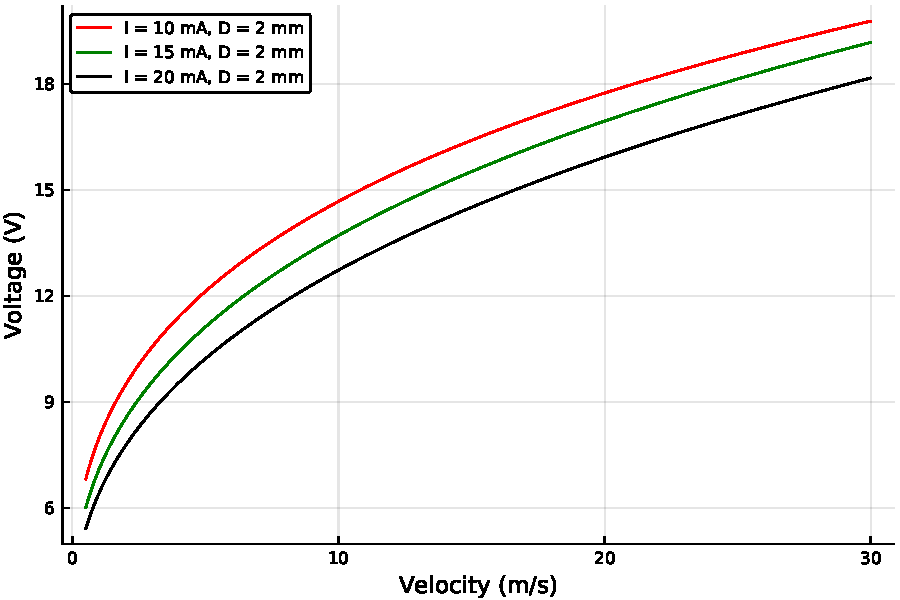
\includegraphics[width=0.45\textwidth]{../../figures/CCA-Eo.pdf} & 
    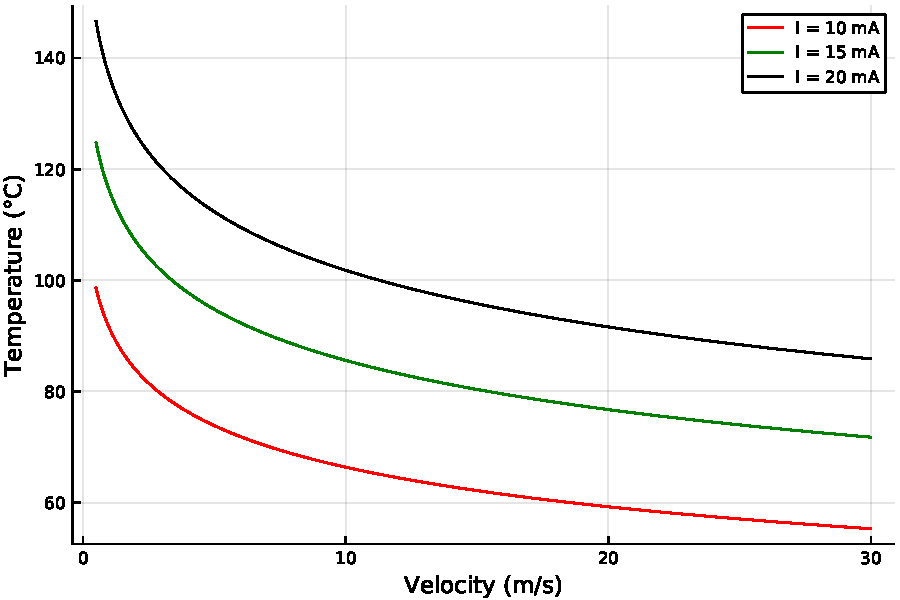
\includegraphics[width=0.45\textwidth]{../../figures/CCA-T.pdf} \\
    \parbox{0.4\textwidth}{\footnotesize (a) Effects of probe current on anemometer output} & \parbox{0.4\textwidth}{\footnotesize (b) Temperature of a thermistor for constant current operation}\\
  \end{tabular}
\end{frame}



\begin{frame}
  \frametitle{Termo-anemômetro a temperatura constante (CTA)}
  \framesubtitle{CTA Pulsado}
  \centering
  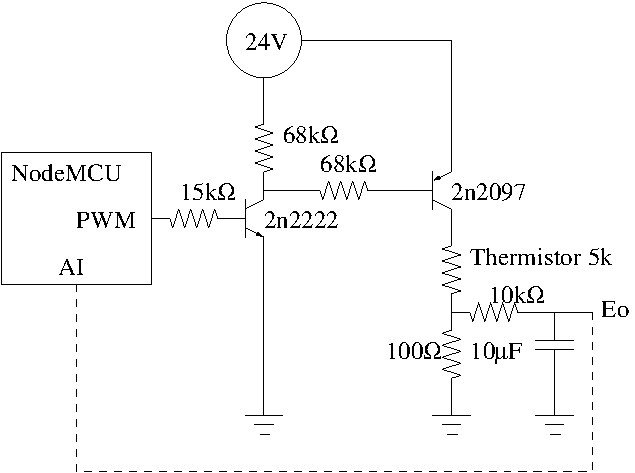
\includegraphics[width=0.66\textwidth]{../../figures/cta.pdf} 
  
\end{frame}

\begin{frame}
  \frametitle{Termo-anemômetro a temperatura constante (CTA)}
  \framesubtitle{Simulação da operação}
 \centering
 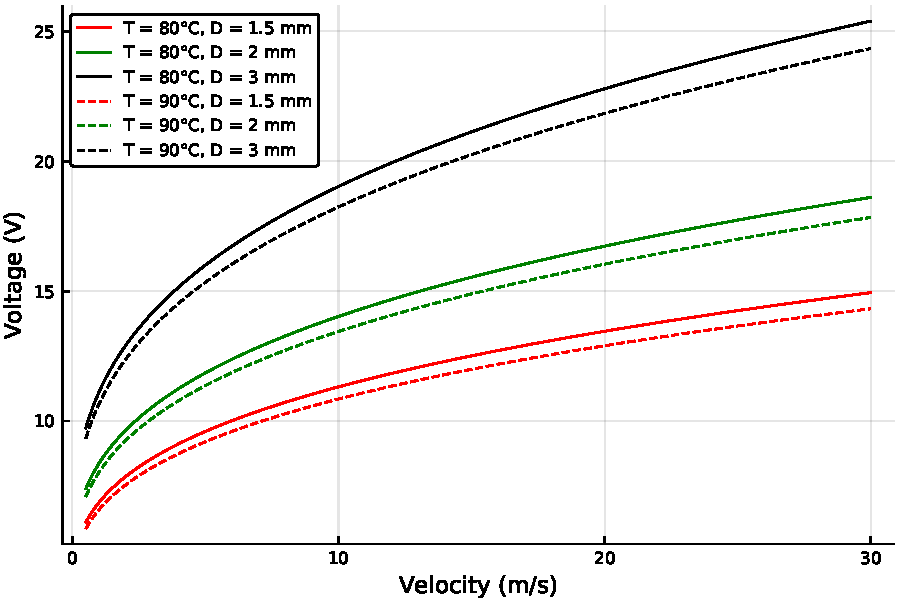
\includegraphics[width=0.9\textwidth]{../../figures/CTA-Eo.pdf} & 
\end{frame}



\begin{frame}
  \frametitle{Calibração e operação do termo-anemômetro a corrente constante (CCA)}
  \centering
  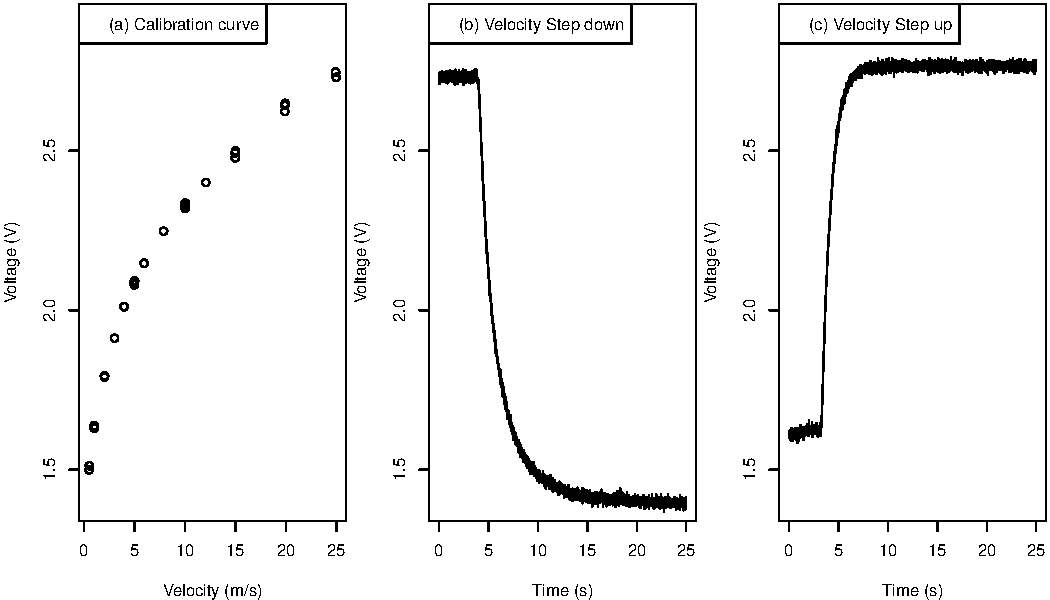
\includegraphics[width=0.95\textwidth]{../../figures/cca-cal.pdf}

 
\end{frame}

\begin{frame}
  \frametitle{Calibração e operação do termo-anemômetro a temperatura constante (CTA)}
  \centering
  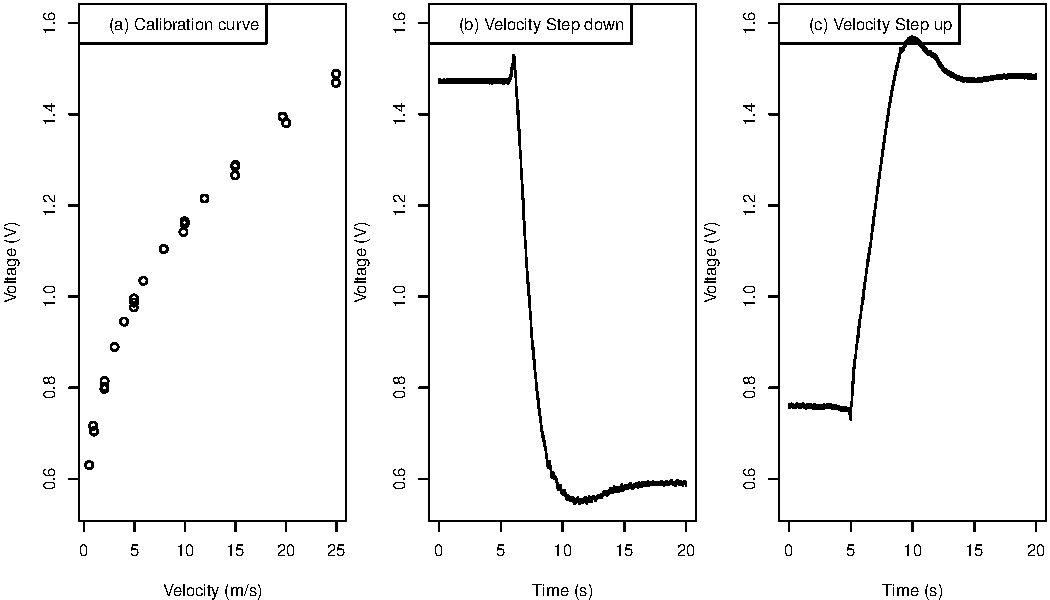
\includegraphics[width=0.95\textwidth]{../../figures/cta-cal.pdf}
 
\end{frame}

\begin{frame}
  \frametitle{Calibração direcional}
  \framesubtitle{Um sensor Omni-direcional?}
  \centering
  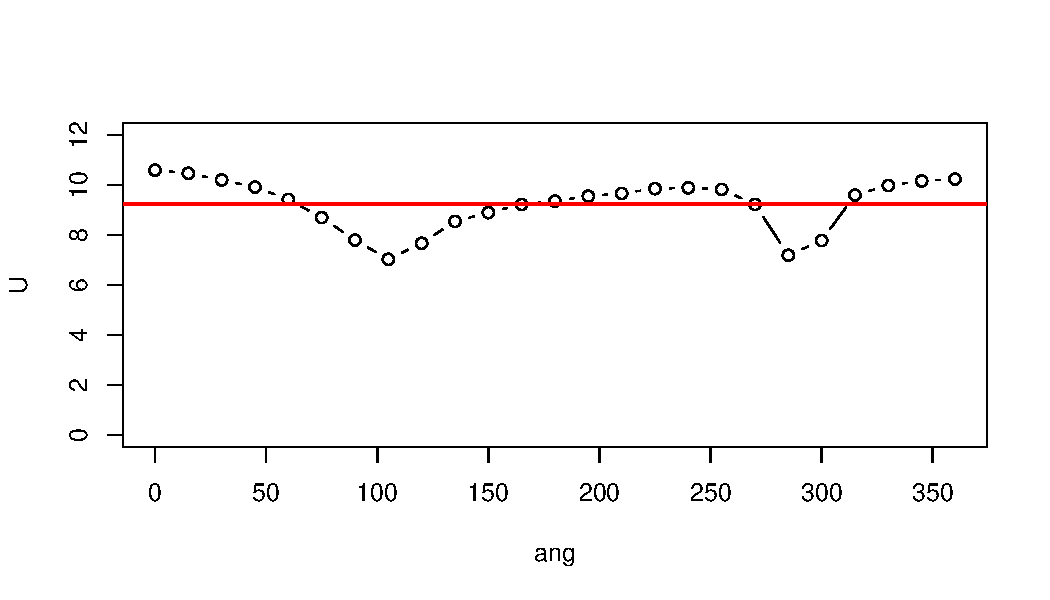
\includegraphics[width=1\textwidth]{../../figures/dircal.pdf}
 
\end{frame}


\begin{frame}
  \frametitle{Multi-sensor CCA}
  \centering
  \begin{tabular}{c}
    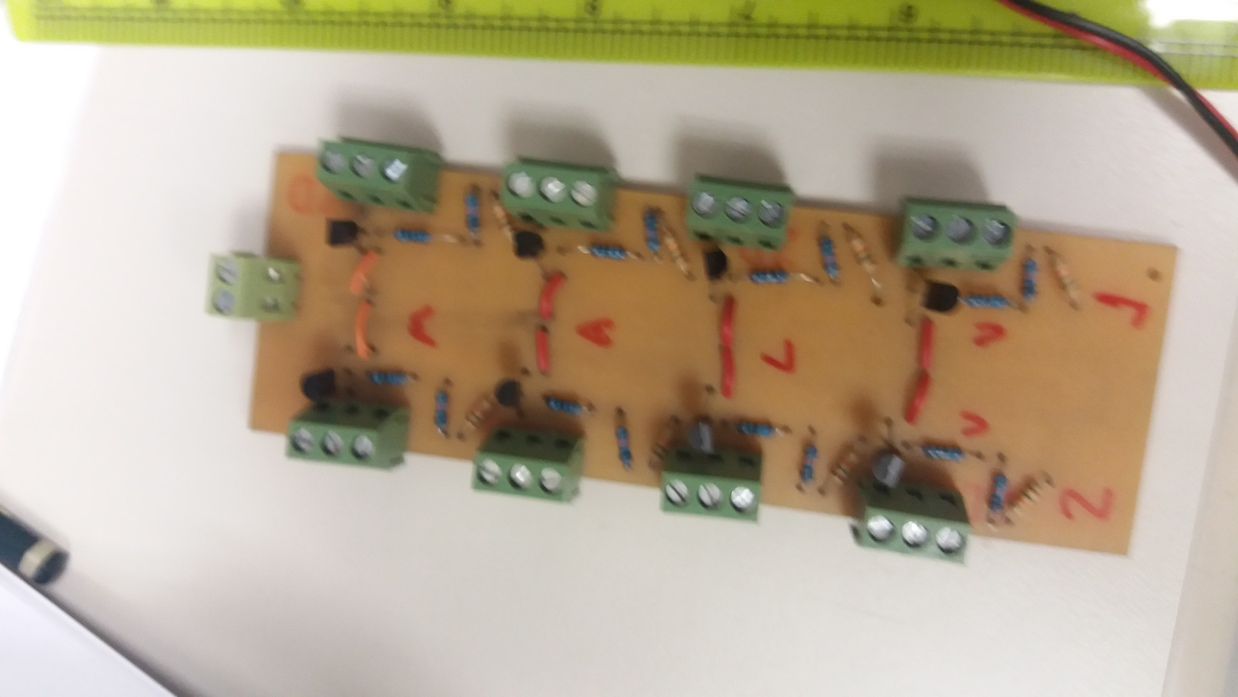
\includegraphics[width=0.75\textwidth]{20181106_192208.jpg}\\
    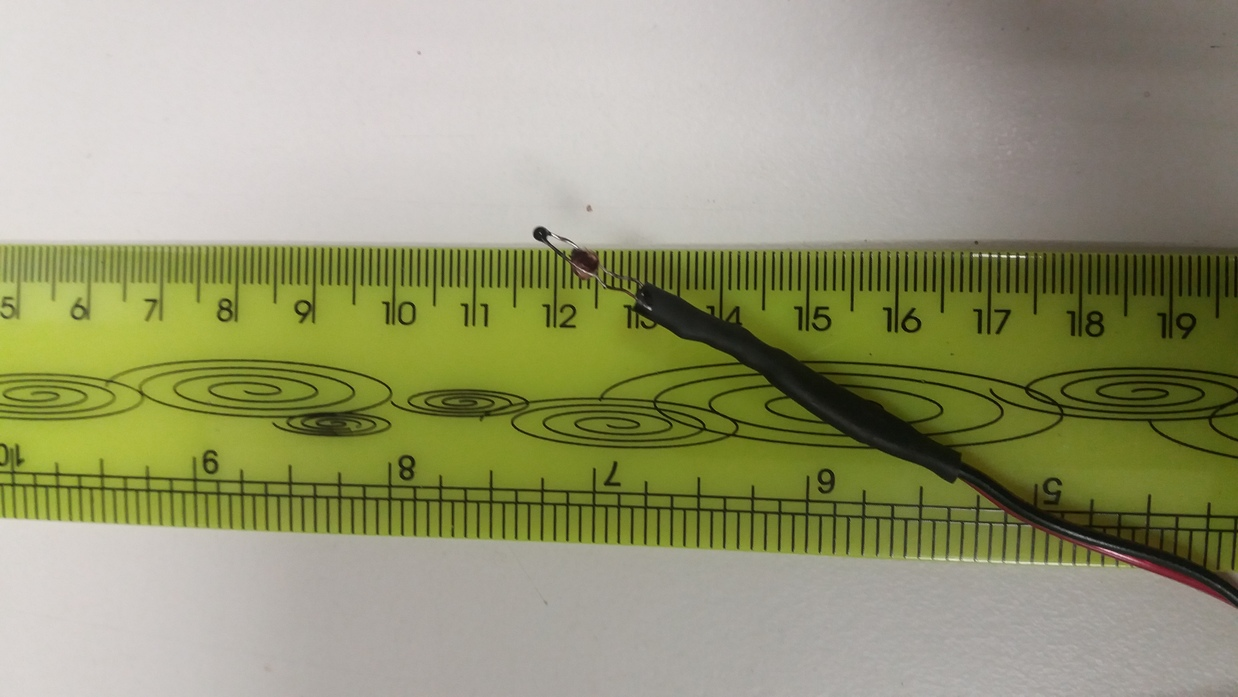
\includegraphics[width=0.75\textwidth]{20181106_192224.jpg}
  \end{tabular}
\end{frame}

\begin{frame}
  \frametitle{Microcontrolador}
  \framesubtitle{Nodemcu 32s}
  \centering
  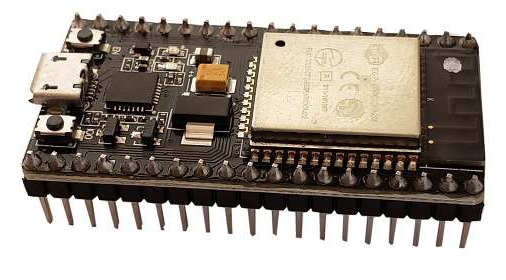
\includegraphics[width=0.6\textwidth]{nodemcu32s.jpg}\\
\end{frame}

\begin{frame}
  \frametitle{Conclusões e discussão}

  \begin{itemize}
  \item O objetivo básico foi alcançado: temos um sistema simples e barato
  \item Inúmeras aplicações podem ser imaginadas!
  \item A simplicidade da eletrônica do CCA é realmente um atrativo
  \item O CTA pulsado é interessante e novo mas o controlador precisa ser melhorado
  \item Qual a robustez dos sensores?
  \item Testar outras geometrias de termistores
  \item Desenvolvimento aberto em \url{https://github.com/pjabardo/ThermistorHW.jl}
  \end{itemize}
\end{frame}

    
  
    
      
  
% ---------------------------------------------------------------
\end{document}
